\paragraph{Exercise 1}
Find the minimum state automaton accepting the language denoted by the regular expression: \code{(ab*\|b*a)*}
\begin{figure}[H]
    \centerline{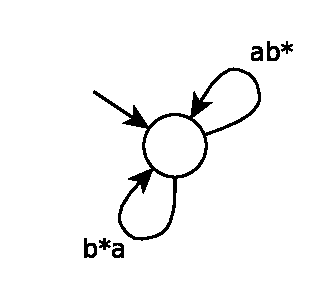
\includegraphics[width=0.3\textwidth]{img/40.pdf}}
\end{figure}
$$
    \Downarrow
$$
\begin{figure}[H]
    \centerline{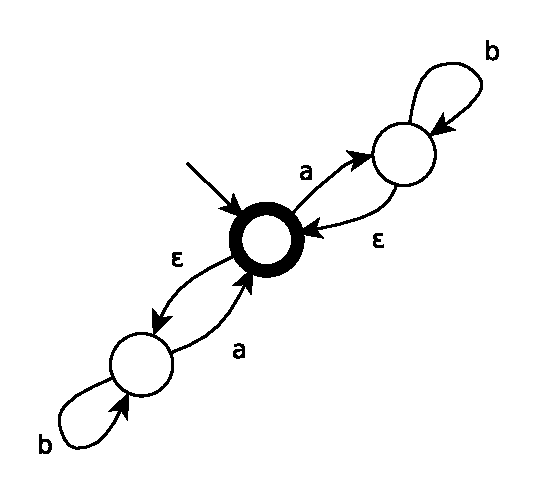
\includegraphics[width=0.5\textwidth]{img/41.pdf}}
\end{figure}
$$
    \Downarrow NFA
$$
\begin{figure}[H]
    \centerline{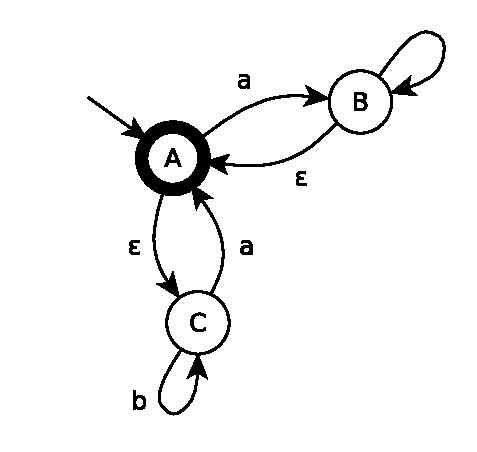
\includegraphics[width=0.4\textwidth]{img/42.pdf}}
\end{figure}
$$
    \Downarrow DFA
$$
\begin{table}[H]
    \centering
    \begin{tabular}{l|l|l}
        & a & b \\ \hline
        A, B & B, A, C & C \\ \hline
        B, A, C & B, A, C & B, A, C \\ \hline
        C & A, C & C \\
    \end{tabular}
\end{table}
$$
    \Downarrow DFA
$$
\begin{figure}[H]
    \centerline{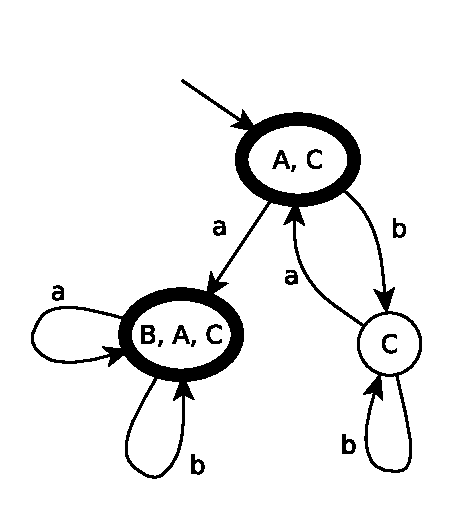
\includegraphics[width=0.3\textwidth]{img/43.pdf}}
\end{figure}
This automaton is already minimum.

\paragraph{Exercise 2}
Verify the equivalence between the following grammars:
\begin{enumerate}
    \item
    $S \to Aa \; | \; Ab \; | \; Sb \; | \; a \; | \; b$ \newline
    $A \to Sa$
    \item
    $S \to aA \; | \; bA \; | \; a \; | \; b$ \newline
    $A \to aS \; | \; bA \; | \; b$
\end{enumerate}

\begin{enumerate}
    \item
    Left regular grammar
    \begin{figure}[H]
        \centerline{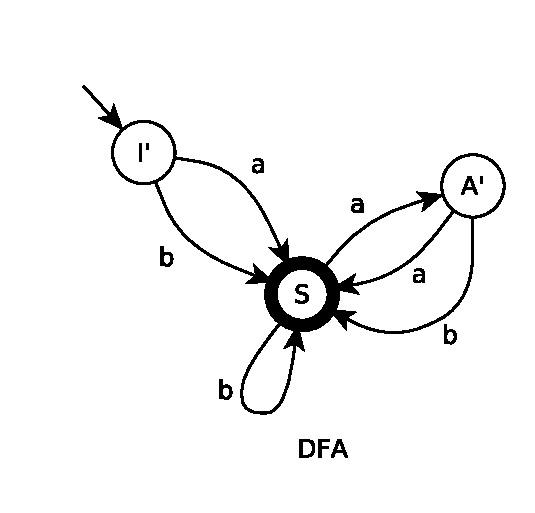
\includegraphics[width=0.4\textwidth]{img/44.pdf}}
    \end{figure}
    $$
        \{I', A', S\}; \{S', B\}
    $$
    \begin{figure}[H]
        \centerline{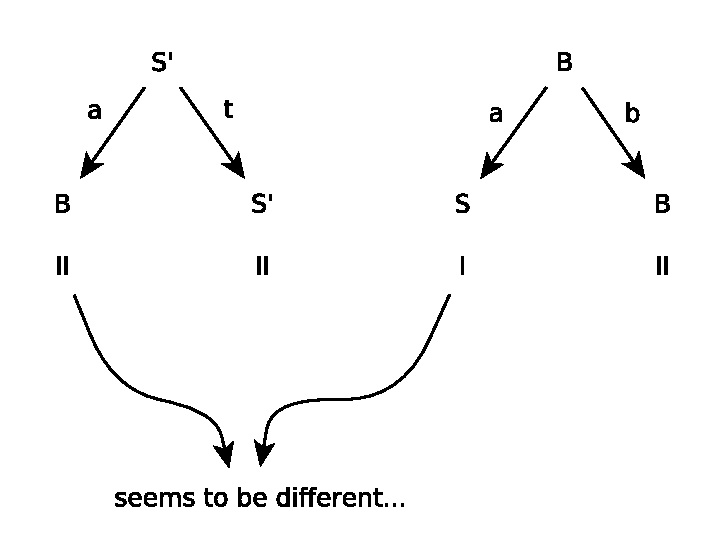
\includegraphics[width=0.3\textwidth]{img/45.pdf}}
    \end{figure}
    \item
    Right regular grammar
    % \begin{figure}[H]
    %     \centerline{\includegraphics[width=0.3\textwidth]{img/46.pdf}}
    % \end{figure}
    \begin{table}[H]
        \centering
        \begin{tabular}{l|l|l}
            & a & b \\ \hline
            S & A, $\Omega$ & A, $\Omega$ \\ \hline
            A, $\Omega$ & S & A, $\Omega$ \\
        \end{tabular}
    \end{table}
    % \begin{figure}[H]
    %     \centerline{\includegraphics[width=0.3\textwidth]{img/47.pdf}}
    % \end{figure}
\end{enumerate}

\paragraph{Exercise 3}
\paragraph{Exercise 4}
\paragraph{Exercise 5}
\paragraph{Exercise 6}
\paragraph{Exercise 7}
\paragraph{Exercise 8}
\paragraph{Exercise 9}
\paragraph{Exercise 10}
\paragraph{Exercise 11}
\paragraph{Exercise 12}
\paragraph{Exercise 13}
\paragraph{Exercise 14}
\paragraph{Exercise 15}
\paragraph{Exercise 16}
\paragraph{Exercise 17}
\paragraph{Exercise 18}
\paragraph{Exercise 19}
\paragraph{Exercise 20}
\paragraph{Exercise 21}
\paragraph{Exercise 22}
\paragraph{Exercise 23}
\paragraph{Exercise 24}
\paragraph{Exercise 25}
\paragraph{Exercise 26}
\paragraph{Exercise 27}
\paragraph{Exercise 28}
\paragraph{Exercise 29}
\paragraph{Exercise 30}
\paragraph{Exercise 31}
\paragraph{Exercise 32}
\paragraph{Exercise 33}
\paragraph{Exercise 34}
\paragraph{Exercise 35}
\paragraph{Exercise 36}
\paragraph{Exercise 37}
\paragraph{Exercise 38}
\paragraph{Exercise 39}
\paragraph{Exercise 40}
\paragraph{Exercise 41}
\paragraph{Exercise 42}
\paragraph{Exercise 43}
\paragraph{Exercise 44}
\paragraph{Exercise 45}
\paragraph{Exercise 46}
\paragraph{Exercise 47}
\paragraph{Exercise 48}
\paragraph{Exercise 49}
\paragraph{Exercise 50}
\paragraph{Exercise 51}
\paragraph{Exercise 52}
\paragraph{Exercise 53}
\paragraph{Exercise 54}
\paragraph{Exercise 55}
\paragraph{Exercise 56}
\paragraph{Exercise 57}
\paragraph{Exercise 58}
\paragraph{Exercise 59}
\paragraph{Exercise 60}
\paragraph{Exercise 61}
\paragraph{Exercise 62}
\paragraph{Exercise 63}
\paragraph{Exercise 64}
\paragraph{Exercise 65}
\paragraph{Exercise 66}
\paragraph{Exercise 67}
\paragraph{Exercise 68}
\paragraph{Exercise 69}
\paragraph{Exercise 70}
\paragraph{Exercise 71}
\paragraph{Exercise 72}
\paragraph{Exercise 73}
\paragraph{Exercise 74}
\paragraph{Exercise 75}
\paragraph{Exercise 76}
\paragraph{Exercise 77}
\paragraph{Exercise 78}
\paragraph{Exercise 79}
\paragraph{Exercise 80}
\paragraph{Exercise 81}
\paragraph{Exercise 82}
\paragraph{Exercise 83}
\paragraph{Exercise 84}
\paragraph{Exercise 85}
\paragraph{Exercise 86}
\paragraph{Exercise 87}
\paragraph{Exercise 88}
\paragraph{Exercise 89}
\paragraph{Exercise 90}
\paragraph{Exercise 91}
\paragraph{Exercise 92}
\paragraph{Exercise 93}
\paragraph{Exercise 94}
\paragraph{Exercise 95}
\paragraph{Exercise 96}
\paragraph{Exercise 97}
\paragraph{Exercise 98}
\paragraph{Exercise 99}
\paragraph{Exercise 100}